\documentclass[12pt]{article} %you must choose a document class
% LTeX: enabled=false
\usepackage{color,graphicx} %allows use of postscript graphics and color output
\textwidth 170mm
\textheight 210mm
\topmargin 0.0mm
\oddsidemargin 0mm
\evensidemargin 0mm

\usepackage{siunitx}
\sisetup{output-exponent-marker=\ensuremath{\mathrm{e}}}
\usepackage{pdfpages}
\usepackage{amsmath}
\usepackage{amssymb}
\usepackage{amsthm}
\usepackage{multicol}
\usepackage{tabularx}
\usepackage{placeins}
\usepackage{float}
\usepackage{listings}
\usepackage[utf8]{inputenc}
\usepackage{mdframed}
\usepackage{graphics}
\usepackage{xspace}
\usepackage[skins,breakable]{tcolorbox}
\usepackage{enumitem}
\usepackage[hidelinks]{hyperref}
\usepackage{datetime2}
\DTMsetup{showzone=true}

\usepackage{listings} % turn on to have code
\usepackage{tikz}
\usepackage{tikz-3dplot}


%put solution in a nice little boxes.
\newtcolorbox{solutionbox}[1][]{
	enhanced jigsaw,
	breakable,
	pad at break=1mm,
	interior hidden,
	colframe=black!50!white,
	title=Solution for #1,
	after title={
			\phantomsection
			\addcontentsline{toc}{subsection}{Solution for #1}
		}
}

% allow infinitely many horizontal lines.
\makeatletter
\newcommand{\boxbar}{%

	\begin{tikzpicture}
		\path[use as bounding box] (0,0) -- (\linewidth,0);
		\draw[color=black!50!white,dashed,dash phase=2pt]
		(0-\kvtcb@leftlower-\kvtcb@boxsep,0)--
		(\linewidth+\kvtcb@rightlower+\kvtcb@boxsep,0);
	\end{tikzpicture}%

}
\makeatother

\usepackage{url}


\usepackage{accents}
% Define \ppori as o with tilde underneath
\newcommand{\ppori}[1]{\underaccent{\tilde}{o}_{#1}}

% Define \pv{v} as underlined v and \pc as underlined c.
% physical vector and physical coordinate system.
% pt, or physical tensor have two double lines.
\newcommand{\pv}[1]{\underline{#1}}
\newcommand{\pc}[1]{\underline{#1}}
\newcommand{\pt}[1]{\underline{\underline{#1}}}



\begin{document}						%Start the document. Everything before this is formatting. 

I cannot guarantee correctness, please tell me if there are mistakes and ask if you have questions.

Last updates: \DTMnow

\tableofcontents

\newpage
\section{Exam 2025}
\begin{solutionbox}[Q1-1]
    7  axes of rotation so 7 degrees of freedom.

    When first joint lines up with the third, it is an arm singularity.

    When fifth joint lines up with the 7th joint, it is a wrist singularity.
\end{solutionbox}


\begin{solutionbox}[Q1-2]

    \begin{align*}
        {^0s} & = \frac{1}{3}\begin{bmatrix}
                                 1 \\2\\2
                             \end{bmatrix}       \\
        {^0A} & =e^{\frac{\pi}{4} {^0s}\times}    \\
              & =e^{\frac{\pi}{4} \left(
        \frac{1}{3}\begin{bmatrix}
                       1 \\2\\2
                   \end{bmatrix}
        \right)\times}                            \\
              & =e^{\frac{\pi}{12} \begin{bmatrix}
                                       0  & -2 & 2  \\
                                       2  & 0  & -1 \\
                                       -2 & 1  & 0  \\
                                   \end{bmatrix}} \\
    \end{align*}


    Expand with Rodrigues if there is extra time.:

    \begin{align*}
        {\,^0A} & =e^{\frac{\pi}{12} \begin{bmatrix}
                                         0  & -2 & 2  \\
                                         2  & 0  & -1 \\
                                         -2 & 1  & 0  \\
                                     \end{bmatrix}}                                                                                                                                                                                                                                                                        \\
                & =I
        +\sin(\pi/4)\frac{1}{3}\begin{bmatrix}
                                   0  & -2 & 2  \\
                                   2  & 0  & -1 \\
                                   -2 & 1  & 0  \\
                               \end{bmatrix}
        +(1-\cos(\pi/4))\frac{1}{9}\begin{bmatrix}
                                       -8 & 2  & 2  \\
                                       2  & -5 & 4  \\
                                       2  & 4  & -5 \\
                                   \end{bmatrix}                                                                                                                                                                                                                                                                          \\
                & =I
        +\frac{\sqrt{2}}{2}\frac{1}{9}\begin{bmatrix}
                                          0  & -6 & 6  \\
                                          6  & 0  & -3 \\
                                          -6 & 3  & 0  \\
                                      \end{bmatrix}
        +(1-\frac{\sqrt{2}}{2})\frac{1}{9}\begin{bmatrix}
                                              -8 & 2  & 2  \\
                                              2  & -5 & 4  \\
                                              2  & 4  & -5 \\
                                          \end{bmatrix}                                                                                                                                                                                                                                                                   \\
                & =\begin{bmatrix}
                       1+(1-\frac{\sqrt{2}}{2})(\frac{-8}{9})                                    & \frac{\sqrt{2}}{2}\cdot(\frac{-6}{9})+(1-\frac{\sqrt{2}}{2})(\frac{2}{9}) & \frac{\sqrt{2}}{2}\cdot(\frac{6}{9})+ (1-\frac{\sqrt{2}}{2})(\frac{2}{9}) \\
                       \frac{\sqrt{2}}{2}\cdot(\frac{6}{9})+(1-\frac{\sqrt{2}}{2})(\frac{2}{9})  & 1+(1-\frac{\sqrt{2}}{2})(\frac{-5}{9})                                    & \frac{\sqrt{2}}{2}\cdot(-3/9)+(1-\frac{\sqrt{2}}{2})(\frac{4}{9})         \\
                       \frac{\sqrt{2}}{2}\cdot(\frac{-6}{9})+(1-\frac{\sqrt{2}}{2})(\frac{2}{9}) & \frac{\sqrt{2}}{2}\cdot(3/9)+(1-\frac{\sqrt{2}}{2})(\frac{4}{9})          & 1+(1-\frac{\sqrt{2}}{2})(\frac{-5}{9})
                   \end{bmatrix} \\
                & =\begin{bmatrix}
                       \frac{1}{9}+\frac{\sqrt{2}}{2}\cdot \frac{8}{9}  & \frac{2}{9}+\frac{\sqrt{2}}{2}\cdot \frac{-8}{9} & \frac{2}{9}+\frac{\sqrt{2}}{2}\cdot\frac{4}{9}  \\
                       \frac{2}{9}+\frac{\sqrt{2}}{2}\cdot \frac{4}{9}  & \frac{4}{9}+\frac{\sqrt{2}}{2}\cdot \frac{5}{9}  & \frac{4}{9}+\frac{\sqrt{2}}{2}\cdot\frac{-7}{9} \\
                       \frac{2}{9}+\frac{\sqrt{2}}{2}\cdot \frac{-8}{9} & \frac{4}{9}+\frac{\sqrt{2}}{2}\cdot \frac{-1}{9} & \frac{4}{9}+\frac{\sqrt{2}}{2}\cdot \frac{5}{9}
                   \end{bmatrix}
    \end{align*}

\end{solutionbox}

\begin{solutionbox}[Q1-3]
    \begin{align*}
        {^1C_0} & = \begin{bmatrix}
                        \cos(\pi/4)  & \sin(\pi/4) & 0 \\
                        -\sin(\pi/4) & \cos(\pi/4) & 0 \\
                        0            & 0           & 1
                    \end{bmatrix}                                       \\
        {^1A}   & =e^{\frac{\pi}{4} {^1s}\times}                                         \\
                & =e^{\frac{\pi}{4} ({^1C_0}{^0s})\times}                                \\
                & =\left(^1C_0\right) e^{\frac{\pi}{4} {^0s}\times} \left(\,^0C_1\right) \\
                & =\left(^1C_0\right) \left(\,^0A\right) \left(\,^1C_0\right)^{T}        \\
    \end{align*}
\end{solutionbox}

\begin{solutionbox}[Q1-3?]
    The question is missing a few words, I'm going to assume that it is given the initial and final, position, velocity and acceleration. And that t goes from 0 to 1.

    \begin{align*}
        P(t)=A+Bt+Ct^2+Dt^3+Et^4+Ft^5 \\
        V(t)=B+2Ct+3Dt^2+4Et^3+5Ft^4  \\
        A(t)=2C+6Dt+12Et^2+20Ft^3
    \end{align*}

    \begin{align*}
        \begin{bmatrix}
            P(0) \\
            V(0) \\
            A(0) \\
            P(1) \\
            V(1) \\
            A(1)
        \end{bmatrix}
         & =
        \begin{bmatrix}
            1 & 0 & 0 & 0 & 0  & 0  \\
            0 & 1 & 0 & 0 & 0  & 0  \\
            0 & 0 & 2 & 0 & 0  & 0  \\
            1 & 1 & 1 & 1 & 1  & 1  \\
            0 & 1 & 2 & 3 & 4  & 5  \\
            0 & 0 & 2 & 6 & 12 & 20 \\
        \end{bmatrix}
        \begin{bmatrix}
            A \\B\\C\\D\\E\\F
        \end{bmatrix} \\
        \begin{bmatrix}
            A \\B\\C\\D\\E\\F
        \end{bmatrix}
         & =
        \begin{bmatrix}
            1 & 0 & 0 & 0 & 0  & 0  \\
            0 & 1 & 0 & 0 & 0  & 0  \\
            0 & 0 & 2 & 0 & 0  & 0  \\
            1 & 1 & 1 & 1 & 1  & 1  \\
            0 & 1 & 2 & 3 & 4  & 5  \\
            0 & 0 & 2 & 6 & 12 & 20 \\
        \end{bmatrix}^{-1}
        \begin{bmatrix}
            P(0) \\
            V(0) \\
            A(0) \\
            P(1) \\
            V(1) \\
            A(1)
        \end{bmatrix}
    \end{align*}

    Solve this for each of the axis separately and coefficient would be shown.

\end{solutionbox}

\begin{solutionbox}[Q1-4]
    \begin{align*}
        T & = \frac{1}{2}m \left(\dot{d_1} - l\sin(\theta_2)\dot{\theta_2}\right)^2 + \frac{1}{2}m\left(l\cos(\theta_2)\dot{\theta_2}\right)^2 + \frac{1}{2}M\dot{d_1}^2                         \\
          & = \frac{1}{2}m \left(\dot{d_1}^2-2\dot{d_1}l\sin(\theta_2)\dot{\theta_2} + l^2\sin^2(\theta_2)\dot{\theta_2}^2 + l^2\cos^2(\theta_2)\dot{\theta_2}^2\right)+ \frac{1}{2}M\dot{d_1}^2 \\
          & = \frac{1}{2}m \left(\dot{d_1}^2-2\dot{d_1}l\sin(\theta_2)\dot{\theta_2} + l^2\dot{\theta_2}^2 \right)+ \frac{1}{2}M\dot{d_1}^2                                                      \\
        V & =mgl\sin(\theta_2)                                                                                                                                                                   \\
    \end{align*}

    \begin{align*}
        L & =T-V                                                                                                                                                \\
        L & =\frac{1}{2}m \left(\dot{d_1}^2-2\dot{d_1}l\sin(\theta_2)\dot{\theta_2} + l^2\dot{\theta_2}^2 \right)+ \frac{1}{2}M\dot{d_1}^2  - mgl\sin(\theta_2) \\
    \end{align*}

    \begin{align*}
        \frac{d}{dt}\left(\frac{\partial L}{\partial \dot{d_1}}\right) - \frac{\partial L}{\partial d_1} & = f_1 \\
        \frac{d}{dt}\left(m\dot{d_1}-ml\sin(\theta_2)\dot{\theta_2}+M\dot{d_1}\right)                    & = f_1 \\
        m\ddot{d_1}-(ml\sin(\theta_2)\ddot{\theta_2}+ml\cos(\theta_2)\dot{\theta_2}^2)+M\ddot{d_1}       & = f_1 \\
        m\ddot{d_1}+M\ddot{d_1}-ml\sin(\theta_2)\ddot{\theta_2}-ml\cos(\theta_2)\dot{\theta_2}^2         & = f_1 \\
        (M+m)\ddot{d_1}-ml\ddot{\theta_2}\sin(\theta_2)-ml\dot{\theta_2}^2\cos(\theta_2)                 & = f_1 \\
    \end{align*}

    \begin{align*}
        \frac{d}{dt}\left(\frac{\partial L}{\partial \dot{\theta_2}}\right) - \frac{\partial L}{\partial \theta_2}                                              & = \tau_2 \\
        \frac{d}{dt}\left(-ml\dot{d_1}\sin(\theta_2)+ ml^2\dot{\theta_2} \right) - \left(-ml\dot{d_1}\cos(\theta_2)\dot{\theta_2} - mgl\cos(\theta_2)\right)    & = \tau_2 \\
        -ml\dot{d_1}\cos(\theta_2)\dot{\theta_2}-ml\ddot{d_1}\sin(\theta_2)+ ml^2\ddot{\theta_2}  + ml\dot{d_1}\cos(\theta_2)\dot{\theta_2} + mgl\cos(\theta_2) & = \tau_2 \\
        -ml\ddot{d_1}\sin(\theta_2)+ ml^2\ddot{\theta_2} + mgl\cos(\theta_2)                                                                                    & = \tau_2 \\
        ml^2\ddot{\theta_2}-ml\ddot{d_1}\sin(\theta_2) + mgl\cos(\theta_2)                                                                                      & = \tau_2 \\
    \end{align*}

\end{solutionbox}

\begin{solutionbox}[Q1-5]
    G term is the terms that only dependent on position
    \begin{align*}
        G(q) = \begin{bmatrix}
                   0 \\
                   mgl\cos(\theta_2)
               \end{bmatrix}
    \end{align*}

    From the process of Lagrangian, terms that multiply with double derivative of position must only be multiplied with terms with no derivative. Just find their factors.
    \begin{align*}
        D(q) = \begin{bmatrix}
                   (M+m)             & -ml\sin(\theta_2) \\
                   -ml\sin(\theta_2) & ml^2
               \end{bmatrix}
    \end{align*}
\end{solutionbox}

\begin{solutionbox}[Q1-6]
    \begin{align*}
        d_0(t)=0                                                             \\
        \dot{d_0}(t)=0                                                       \\
        \ddot{d_0}(t)=0                                                      \\
        \theta_0(t)=-\frac{\pi}{2} \cos\left(\frac{\pi}{T}T\right)           \\
        \dot{\theta_0}(t)= \frac{\pi^2}{2T} \sin\left(\frac{\pi}{T}T\right)  \\
        \ddot{\theta_0}(t)=\frac{\pi^3}{2T^2}\cos\left(\frac{\pi}{T}T\right) \\
    \end{align*}

    \begin{align*}
        f_1 = (M+m)\ddot{d_1}-ml\ddot{\theta_2}\sin(\theta_2)-ml\dot{\theta_2}^2\cos(\theta_2)           \\
        f(t) =-ml\ddot{\theta_0}(t)\sin(\theta_0(t))-ml\left(\dot{\theta_0}(t)\right)^2\cos(\theta_0(t)) \\
    \end{align*}

    \begin{align*}
        \tau_1 = ml^2\ddot{\theta_2}-ml\ddot{d_1}\sin(\theta_2) + mgl\cos(\theta_2) \\
        \tau(t) = ml^2 \ddot{\theta_0}(t) + mgl\cos(\theta_0(t))                    \\
    \end{align*}

    Expansion would take too long, I'm just going to leave it as is.
\end{solutionbox}

\begin{solutionbox}[Q1-7]
    PD plus gravity is in joint space.

    Given desired $q_r$ and desired $\dot{q_r}$. $e_{q} = q_r-q$. $e_{qd} = \dot{q_r}-\dot{q}$. Get gravity term from the term on top, call it $u_g$ (this calculated from measured q). $u=kp\cdot e_q + kv\cdot e_{qd} + u_g$

    PD plus feedforward is the following.

    Given desired $q_r$ and desired $\dot{q_r}$. $e_{q} = q_r-q$. $e_{qd} = \dot{q_r}-\dot{q}$. Get all the torques from the equations of motion and call that $u_{ff}$. (this uses desire $q$, desired $\dot{q}$, and desired $\ddot{q}$) $u=kp\cdot e_q + kv\cdot e_{qd} + u_{ff}$

    PD control is just joint space PD control.

    Task space stiffness control is task space pd control.

    Computed torque control moves the equations of motion into the loop, but input is still joint space. (the process of moving it in also changes the calculation to go from the desired to measured. Why? Because measured is the correct option and the desired is just a good approximation that can be precomputed outside the loop.)

    Resolved acceleration is one step above that and the input is in task space.
\end{solutionbox}

\begin{solutionbox}[Q1-8]
    BFS, no need to detail
\end{solutionbox}

\begin{solutionbox}[Q1-9]

    (i)

    Cameras have different parameters, without calibrating, it is hard to know precisely how a pixel gets mapped to a line in 3d space.

    Extrinsic parameters are like the displacement and orientation of the camera with respect to some references coordinate frame.

    Intrinsic parameters are like the focal length, principal point, field of view, and lens distortion of the camera.

    Single simple projective transform ignores lens distortion.


    (ii)

    Hough transform is an algorithm to process images to identify circle in the image. It is done by transforming each pixel into a circle and added to an accumulator. Then the points in accumulator with high number are likely center of circles. This algorithm can also be used to identify lines. For that, the pixels don't contribute to circles in parameter space but rather inside. Each point in parameter space is a line. Vertical axis is how far the line is from the center and horizontal axis is the angle of the line.

    (iii)

    Corners are pixels in an image that have some saliency or recognizability. a different description is that it is points with large intensity change in multiple directions.

    Binary string descriptors is just the result of brightness comparisons done concatenated into a binary number. It is used in brief to identify image by going over a patch and checking relative brightness changes between some optimized pairs of pixels.

    (iv)

    Closing is first dilating then eroding. Since the dilating process expands the white areas, some small black regions may be completely filled out. Then, in the eroding process expands the back regions back out. But since some black regions are completely erased, they won't come back after eroding. The combined effect is as if the black holes in the image are "closed". Opening works exactly oppositely by First making the black regions larger which erases the small white regions. Then, dilating back returns black region to it previous size, but small white regions in the black regions have been erased or "opened". Alternatively, closing removes pepper and opening removes salt.

    (v)

    A and C can be used as such.

    B is not true, but it can help since it averages out the salt and pepper noise in a sense.

    D is completely false.
\end{solutionbox}

% 130 minutes first pass. 7:20 - 9:30

\newpage
% 2:10

\begin{solutionbox}[Q2-1]

    \begin{center}
        \centering
        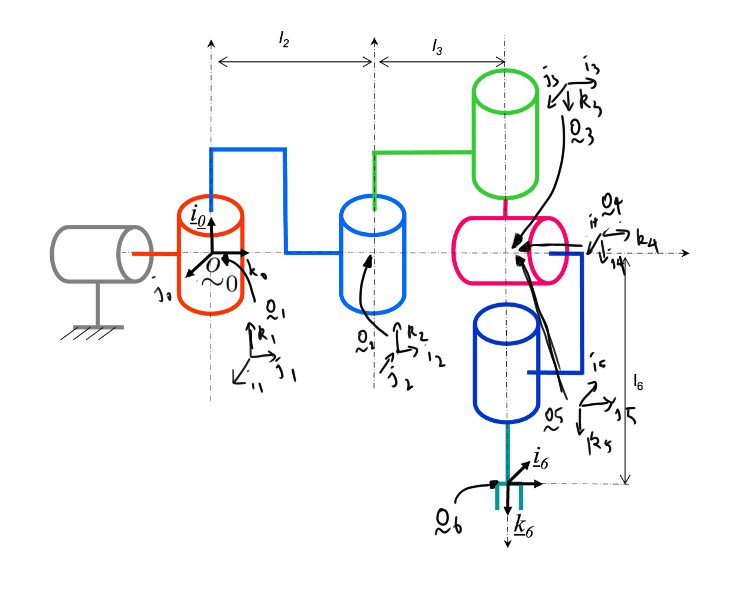
\includegraphics[width=120mm]{imgs/y2025-v1-q2-1.png}
    \end{center}

    \begin{center}
        \begin{tabular}{lllll}
            Link & $\theta$           & $d$   & $a$   & $\alpha$ \\
            1    & $\pi/2 + \theta_1$ & 0     & 0     & $\pi/2$  \\
            2    & $\pi/2+\theta_2$   & 0     & $l_2$ & 0        \\
            3    & $\theta_3$         & 0     & $l_3$ & $\pi$    \\
            4    & $-\pi/2+\theta_4$  & 0     & 0     & $\pi/2$  \\
            5    & $\pi+\theta_5$     & 0     & 0     & $\pi/2$  \\
            6    & $\theta_6$         & $l_6$ & 0     & 0        \\
        \end{tabular}
    \end{center}

    Note link 1 is from gray to red.

    \begin{align*}
        {\,^0T_1} & =
        \begin{bmatrix}
            [e^{\left(\pi/2+\theta_1\right)k\times}] & [0] \\
            [0]                                      & 1
        \end{bmatrix}
        \begin{bmatrix}
            [e^{\left(\pi/2\right)i\times}] & [0] \\
            [0]                             & 1
        \end{bmatrix} \\
                  & =
        \begin{bmatrix}
            [e^{\left(\pi/2+\theta_1\right)k\times} e^{\left(\pi/2\right)i\times}] & [0] \\
            [0]                                                                    & 1
        \end{bmatrix}
    \end{align*}

    \begin{align*}
        {\,^1T_2} & =
        \begin{bmatrix}
            [e^{\left(\pi/2+\theta_2\right)k\times}] & [0] \\
            [0]                                      & 1
        \end{bmatrix}
        \begin{bmatrix}
            [I_3] & [l_2 i] \\
            [0]   & 1
        \end{bmatrix} \\
                  & =
        \begin{bmatrix}
            [e^{\left(\pi/2+\theta_2\right)k\times}] & [l_2 i] \\
            [0]                                      & 1
        \end{bmatrix}
    \end{align*}

    \begin{align*}
        {\,^2T_3} & =
        \begin{bmatrix}
            [e^{\left(\theta_3\right)k\times}] & [0] \\
            [0]                                & 1
        \end{bmatrix}
        \begin{bmatrix}
            [e^{\left(\pi\right)i\times}] & [l_2 i] \\
            [0]                           & 1
        \end{bmatrix} \\
                  & =
        \begin{bmatrix}
            [e^{\left(\theta_3\right)k\times} e^{\left(\pi\right)i\times}] & [e^{\left(\theta_3\right)k\times} l_2 i] \\
            [0]                                                            & 1
        \end{bmatrix}
    \end{align*}

    \begin{align*}
        {\,^3T_4} & =
        \begin{bmatrix}
            [e^{\left(-\pi/2+\theta_4\right)k\times}] & [0] \\
            [0]                                       & 1
        \end{bmatrix}
        \begin{bmatrix}
            [e^{\left(\pi/2\right)i\times}] & [0] \\
            [0]                             & 1
        \end{bmatrix} \\
                  & =
        \begin{bmatrix}
            [e^{\left(-\pi/2+\theta_4\right)k\times} e^{\left(\pi/2\right)i\times}] & [0] \\
            [0]                                                                     & 1
        \end{bmatrix}
    \end{align*}

    \begin{align*}
        {\,^4T_5} & =
        \begin{bmatrix}
            [e^{\left(\pi+\theta_5\right)k\times}] & [0] \\
            [0]                                    & 1
        \end{bmatrix}
        \begin{bmatrix}
            [e^{\left(\pi/2\right)i\times}] & [0] \\
            [0]                             & 1
        \end{bmatrix} \\
                  & =
        \begin{bmatrix}
            [e^{\left(\pi+\theta_5\right)k\times} e^{\left(\pi/2\right)i\times}] & [0] \\
            [0]                                                                  & 1
        \end{bmatrix}
    \end{align*}

    \begin{align*}
        {\,^5T_6} & =
        \begin{bmatrix}
            [e^{\left(\theta_6\right)k\times}] & [l_6k] \\
            [0]                                & 1
        \end{bmatrix}
    \end{align*}
\end{solutionbox}

\begin{solutionbox}[Q2-2]
    \footnotesize
    \begin{align*}
        J & =
        \begin{bmatrix}
            \pv{k}_0\times \left(\ppori{6}-\ppori{0}\right) &
            \pv{k}_1\times \left(\ppori{6}-\ppori{1}\right) &
            \pv{k}_2\times \left(\ppori{6}-\ppori{2}\right) &
            \pv{k}_3\times \left(\ppori{6}-\ppori{3}\right) &
            \pv{k}_4\times \left(\ppori{6}-\ppori{4}\right) &
            \pv{k}_5\times \left(\ppori{6}-\ppori{5}\right)   \\
            \pv{k}_0                                        &
            \pv{k}_1                                        &
            \pv{k}_2                                        &
            \pv{k}_3                                        &
            \pv{k}_4                                        &
            \pv{k}_5
        \end{bmatrix}
    \end{align*}
    \normalsize

    Since $\ppori{3} = \ppori{4}=\ppori{5}$, left multiply with $$$$

    \begin{align*}
        \begin{bmatrix}
            I & \left(\ppori{6}-\ppori{3}\right)\times \\
            0 & I
        \end{bmatrix} J & =
        \begin{bmatrix}
            \pv{k}_0\times \left(\ppori{3}-\ppori{0}\right) &
            \pv{k}_1\times \left(\ppori{3}-\ppori{1}\right) &
            \pv{k}_2\times \left(\ppori{3}-\ppori{2}\right) & 0 & 0 & 0 \\
            \pv{k}_0                                        &
            \pv{k}_1                                        &
            \pv{k}_2                                        &
            \pv{k}_3                                        &
            \pv{k}_4                                        &
            \pv{k}_5
        \end{bmatrix}
    \end{align*}

    Then the system can be analyzed with arm and wrist singularity separately.

    Arm singularity arise when o3 is in the line formed by o0 and k0.

    Wrist singularity when k3 and k5 are inline of $\theta_4=0$

\end{solutionbox}

\begin{solutionbox}[Q2-3]
    Since q0 and q1 can reach point i2 in any direction and the rest can extend l2+l3+l6 away from o0. Then the reachable workspace must have an outer bound of a sphere with radius l2+l3+l6 centered at o0.

    The inner radius of the sphere would be the longest arm minus the two smaller arms and if that is negative, the minimum radius is 0. Expressed mathematically:

    $\max(\max(l2,l3,l6)-(l2+l3+l6 - \max(l2,l3,l6)),0) = \max(2\max(l2,l3,l6)-l2-l3-l6,0)$
\end{solutionbox}

\begin{solutionbox}[Q2-4]
    Due to the spherical wrist, the geometry of the arm and that of the wrist can be analyzed independently.

    There are going to be 8 solutions and I will be referring to them as binaries encoding since they are natural.

    Wrist center is at $\ppori{6}-l6 \pv{k}_6$.

    For o3 to be there, there are four solutions to the arm.

    First project $\ppori{3}-\ppori{0}$ onto the vector $\pv{k}_0$ to get $\left(\ppori{3}-\ppori{0}\right) \parallel \pv{k}_0 = \left(\ppori{3}-\ppori{0}\right) \cdot \pv{k}_0$.

    Then subtract it off from $\ppori{3}-\ppori{0}$ to get  $\left(\ppori{3}-\ppori{0}\right) \perp \pv{k}_0 = \left(\ppori{3}-\ppori{0}\right) - \left(\ppori{3}-\ppori{0}\right) \cdot \pv{k}_0 \pv{k}_0$

    Then use Kahan p1 with $s = j0$ and $t = \left(\ppori{3}-\ppori{0}\right) \perp \pv{k}_0$. Let the result be $\left|\theta_{0-v0}\right|$ This give the absolute value of the angle of $\theta_0$ for half of the solutions.

    The sign of $\theta_{0-v0}$ is the same as $ - \left(\ppori{3}-\ppori{0}\right) \cdot \pv{i}_0$.

    The other version of the solution, $\theta_{0-v0}$ is $\theta_{0-v0}+\pi$

    For each solution, calculate the mean angle for $\theta_2$ which is by removing the component of $\left(\ppori{3}-\ppori{0}\right)$ that is perpendicular to $\pv{k}_1$ and using Kahan P1 between that and $\pv{j}_1$ to find the absolute value of angle to move by. Then use dot product between $\left(\ppori{3}-\ppori{0}\right)$ and $-\pv{i}_1$ to determine the sign. This mean angle changes with which solution is being used for $theta_1$

    The delta from the mean is $\pi - \text{Kahan P4}(a=\left|\ppori{3}-\ppori{0}\right|,b=l_2,c=l_3)$.

    Then, using Kahan p4 with a=l2, b=l3, and c = $\left|\ppori{3}-\ppori{0}\right|$, the absolute value of theta 3 can be found.

    The first solution is then $\theta_2 = \text{mean} + \text{delta}$ and $\theta_3 = -\left|\theta_3\right|$. And the second solution is $\theta_2 = \text{mean} - \text{delta}$ and $\theta_3 = \left|\theta_3\right|$

    Lastly is the wrist orientation. For any given combination of theta 1, 2, and 3, $\ppori{3}$ and $\pc{C}_3$ are set.

    Project k5 onto i3 and j3, calculate the angle formed between $j_3$ and the projection gives $theta_4$. There are two solutions $\pi$ apart.

    Use Kahan p2, u is k3, w is k5, s is k4, solves for theta 4.

    Use Kahan p2, u is i5, w is i6, s is k5 or k6, solves for theta 5.

    % 40 minutes on this alone
\end{solutionbox}


\begin{solutionbox}[Q2-4 alternatively]
    \begin{center}
        \centering
        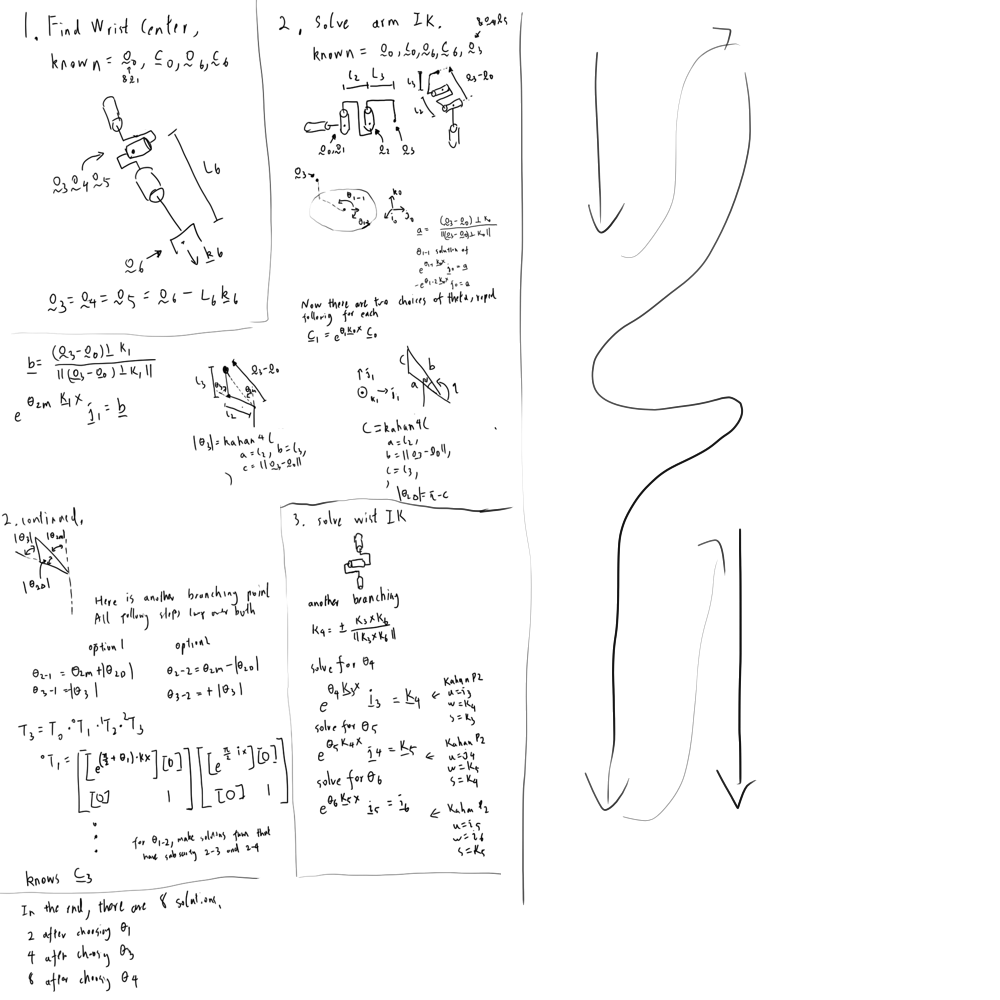
\includegraphics[width=\textwidth]{imgs/y2025-v1-q2-4.png}
    \end{center}
\end{solutionbox}

\begin{solutionbox}[Q2-4?]
    This is a task space stiffness controller.


    \begin{align*}
        {^0\delta_x} = x_r-x              \\
        {\,^0F} = {\,^0K_p}{\,^0\delta x} \\
        \tau=J^T {\,^0F}                  \\
    \end{align*}

    \begin{align*}
        {^0\delta_x} = x_r-x                     \\
        {\,^s\delta x} ={\,^sC_0} {\,^0\delta x} \\
        {\,^sF} = {\,^sK_p}{\,^s\delta x}        \\
        {\,^0F} = {\,^0C_s}{\,^sF}               \\
        \tau=J^T {\,^0F}                         \\
    \end{align*}

    % 4:15
\end{solutionbox}


\newpage
\section{Exam 2024}
% 7:10
% -50

\begin{solutionbox}[Q1-1]
    \begin{center}
        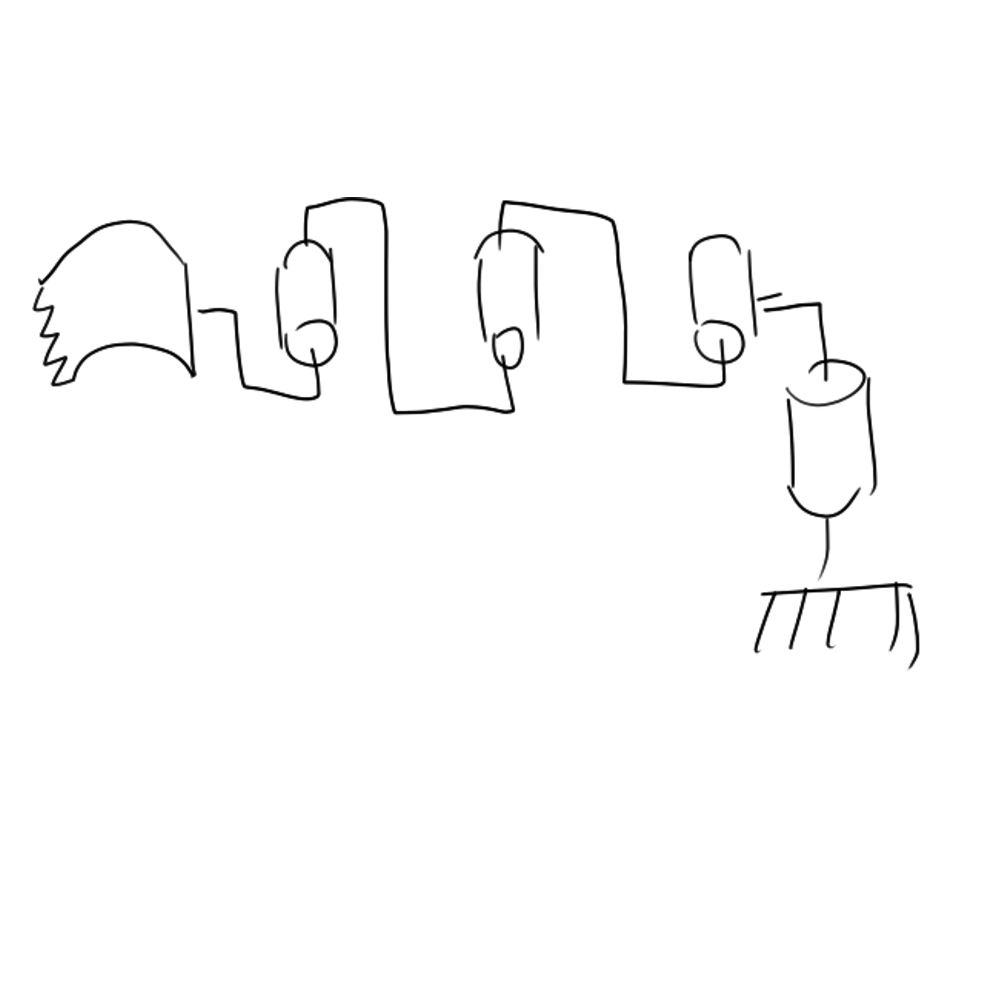
\includegraphics[width=120mm]{imgs/y2024-v1-q1-1.png}
    \end{center}
\end{solutionbox}


\begin{solutionbox}[Q1-2]
    \begin{align*}
        {\,^5\omega_{6,5}}      & = \dot{\theta_6} k                                                                                       \\
        {\pv{\omega}_{6,5}}     & = \pc{C}_5 \dot{\theta_6} k                                                                              \\
        {\pv{\omega}_{6,5}}     & = \pc{C}_4 e^{\theta_5 k\times}e^{-\psi i\times} \dot{\theta_6} k                                        \\
        {\pv{\omega}_{6,5}}     & = \pc{C}_3 e^{\theta_4 k\times} e^{\psi i \times} e^{\theta_5 k\times}e^{-\psi i\times} \dot{\theta_6} k \\
        {\,^3\pv{\omega}_{6,5}} & =e^{\theta_4 k\times} e^{\psi i \times} e^{\theta_5 k\times}e^{-\psi i\times} \dot{\theta_6} k           \\
    \end{align*}

    \begin{align*}
        {\,^4\omega_{5,4}}      & = \dot{\theta_5} k                                                 \\
        {\pv{\omega}_{5,4}}     & = \pc{C}_4 \dot{\theta_5} k                                        \\
        {\pv{\omega}_{5,4}}     & = \pc{C}_3 e^{\theta_4 k\times} e^{\psi i \times} \dot{\theta_5} k \\
        {\,^3\pv{\omega}_{5,4}} & =e^{\theta_4 k\times} e^{\psi i \times} \dot{\theta_5} k           \\
    \end{align*}
    \begin{align*}
        {\,^3\omega_{4,3}} & = \dot{\theta_3} k \\
    \end{align*}

    \begin{align*}
        {\,^3\omega_{6,3}} & ={\,^3\omega_{6,5}}  + {\,^3\omega_{5,4}}  + {\,^3\omega_{4,3}}                                                                           \\
        {\,^3\omega_{6,3}} & =  \dot{\theta_3} k + e^{\theta_4 k\times} e^{\psi i \times} ( \dot{\theta_5} k +e^{\theta_5 k\times}e^{-\psi i\times} \dot{\theta_6} k ) \\
    \end{align*}


\end{solutionbox}

\begin{solutionbox}[Q1-3]

    The question is identical to that in Exam 2025.

    I think there is still value so i redid it with different working.

    First find the direction to move the end effector to move from $\ppori{a}$ to $\ppori{b}$ which is $(\ppori{b}-\ppori{a})$.

    Second find the axis and angle to rotate such that the effector rotates from $\pc{C}_a$ to $\pc{C}_b$.

    Third, decide the profile to move by. This is the step where quintic polynomial comes in as it is the minimum number of degrees such that the initial and final position, velocity, and acceleration can be independently set.

    Forth, at every time step, compute the inverse kinematics from for the position and orientation at that time stamps.

    The first three steps can be written as the following.
    \begin{align*}
        \ppori{t} = \ppori{a} + s(t) (\ppori{b}-\ppori{a}) \\
        \pc{C}_t = Rot(\pc{C}_a,\hat{u},s(t)\theta)        \\
    \end{align*}
    Where $\pc{C}_b = e^{\theta \hat{u}} \pc{C}_a$, and $s(t)=0$ at $t=0$ and $s(t)=1$ at $t=t_f$.

\end{solutionbox}

\begin{solutionbox}[Q1-4]
    The following should be identical to that in Exam 2025.

    I think there is still value so i redid it.

    \begin{align*}
        T & =\frac{1}{2}M\dot{d_1}^2 + \frac{1}{2}m(\dot{d_1}-l\dot{\theta_2}\sin(\theta_2))^2+\frac{1}{2}m(l\dot{\theta_2}\cos(\theta_2))^2                                              \\
          & =\frac{1}{2}M\dot{d_1}^2 + \frac{1}{2}m\left((\dot{d_1})^2-2l\dot{d_1}\dot{\theta_2}\sin(\theta_2)+(l\dot{\theta_2}\sin(\theta_2))^2+(l\dot{\theta_2}\cos(\theta_2))^2\right) \\
          & =\frac{1}{2}M\dot{d_1}^2 + \frac{1}{2}m\left((\dot{d_1})^2-2l\dot{d_1}\dot{\theta_2}\sin(\theta_2)+(l\dot{\theta_2})^2 \right)                                                \\
          & =\frac{1}{2}(M+m)\dot{d_1}^2 + \frac{1}{2}m\left(-2l\dot{d_1}\dot{\theta_2}\sin(\theta_2)+(l\dot{\theta_2})^2 \right)                                                         \\
        V & =mgl\sin(\theta_2)
    \end{align*}

    \begin{align*}
        L & =T-V                                                                                                                                    \\
          & =\frac{1}{2}(M+m)\dot{d_1}^2 + \frac{1}{2}m\left(-2l\dot{d_1}\dot{\theta_2}\sin(\theta_2)+(l\dot{\theta_2})^2 \right)-mgl\sin(\theta_2) \\
    \end{align*}

    \begin{align*}
        \frac{d}{dt} \left(\frac{\partial L}{\partial \dot{d_1}} \right) - \frac{\partial L}{\partial d_1} & = f_1 \\
        \frac{d}{dt} \left( (M+m)\dot{d_1} -ml\dot{\theta_2}\sin(\theta_2) \right) -0                      & = f_1 \\
        (M+m)\ddot{d_1} -ml\ddot{\theta_2}\sin(\theta_2)-ml\dot{\theta_2}^2\cos(\theta_2)                  & = f_1 \\
    \end{align*}

    \begin{align*}
        \frac{d}{dt} \left(\frac{\partial L}{\partial \dot{\theta_2}} \right) - \frac{\partial L}{\partial \theta_2}                                        & = \tau_2 \\
        \frac{d}{dt} \left(-ml\dot{d_1}\sin(\theta_2)+ml^2\dot{\theta_2} \right) - (-ml\dot{d_1}\dot{\theta_2}\cos(\theta_2)-mgl\cos(\theta_2))             & = \tau_2 \\
        -ml\ddot{d_1}\sin(\theta_2)-ml\dot{d_1}\dot{\theta_2}\cos(\theta_2)+ml^2\ddot{\theta_2} +ml\dot{d_1}\dot{\theta_2}\cos(\theta_2)+ mgl\cos(\theta_2) & = \tau_2 \\
        ml^2\ddot{\theta_2}-ml\ddot{d_1}\sin(\theta_2) + mgl\cos(\theta_2)                                                                                  & = \tau_2 \\
    \end{align*}

\end{solutionbox}

\begin{solutionbox}[Q1-5]
    The following should be identical to that in Exam 2025.

    I think there is still value so i redid it.

    \begin{align*}
        G(q)=
        \begin{bmatrix}
            0 \\
            mgl\cos(\theta_2)
        \end{bmatrix}
    \end{align*}

    \begin{align*}
        D(q) =
        \begin{bmatrix}
            M+m               & -ml\sin(\theta_2) \\
            -ml\sin(\theta_2) & ml^2
        \end{bmatrix}
    \end{align*}

\end{solutionbox}

\begin{solutionbox}[Q1-6]
    The following should be identical to that in Exam 2025.

    I think there is still value so i redid it.

    \begin{align*}
        d_0(t)=0                                                  \\
        \dot{d}_0(t)=0                                            \\
        \ddot{d}_0(t)=0                                           \\
        \theta_0(t)=\frac{-\pi}{2}\cos(\frac{\pi}{T}t)            \\
        \dot{\theta}_0(t)=\frac{\pi^2}{2T}\sin(\frac{\pi}{T}t)    \\\
        \ddot{\theta}_0(t)=\frac{\pi^3}{2T^2}\cos(\frac{\pi}{T}t) \\\
    \end{align*}

    \begin{align*}
        \tau_2 & = ml^2\ddot{\theta_2}-ml\ddot{d_1}\sin(\theta_2) + mgl\cos(\theta_2)                                                 \\
        \tau_2 & = ml^2\left[\frac{\pi^3}{2T^2}\cos(\frac{\pi}{T}t)\right] + mgl\cos(\left[\frac{-\pi}{2}\cos(\frac{\pi}{T}t)\right]) \\
        f_1    & = (M+m)\ddot{d_1} -ml\ddot{\theta_2}\sin(\theta_2)-ml\dot{\theta_2}^2\cos(\theta_2)                                  \\
        f_1    & =
        -ml\left[\frac{\pi^3}{2T^2}\cos(\frac{\pi}{T}t)\right]
        \sin(\left[\frac{-\pi}{2}\cos(\frac{\pi}{T}t)\right])
        -ml\left[\frac{\pi^2}{2T}\sin(\frac{\pi}{T}t)\right]^2
        \cos(\left[\frac{-\pi}{2}\cos(\frac{\pi}{T}t)\right])                                                                         \\
    \end{align*}
\end{solutionbox}

\begin{solutionbox}[Q1-7]
    see Exam 2025 q1-7.
\end{solutionbox}

\begin{solutionbox}[Q1-8]
    see Exam 2025 q1-8.
\end{solutionbox}

\begin{solutionbox}[Q1-9]
    see Exam 2025 q1-9.
\end{solutionbox}
\newpage


\begin{solutionbox}[Q2-1]
    See Exam 2025 q2-1.
\end{solutionbox}

\begin{solutionbox}[Q2-2]
    See Exam 2025 q2-2.
\end{solutionbox}

\begin{solutionbox}[Q2-3]
    See Exam 2025 q2-3.
\end{solutionbox}

\begin{solutionbox}[Q2-4]
    See Exam 2025 q2-4.
\end{solutionbox}

\begin{solutionbox}[Q2-5]
    See Exam 2025 q2-5.
\end{solutionbox}

\newpage
\section{Exam 2023}
% 4:05 - 5:05
% 60 minutes

\begin{solutionbox}[Q1-1]

    \begin{center}
        \centering
        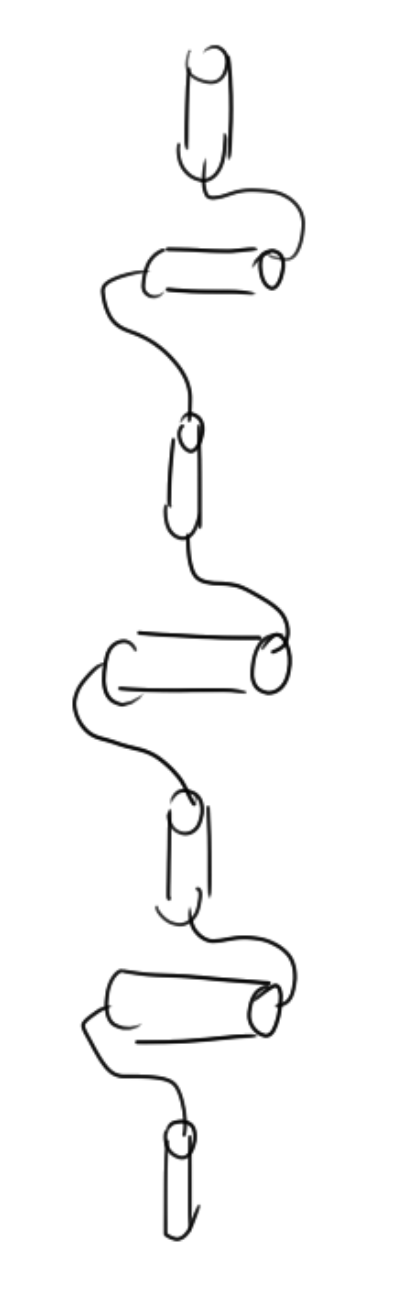
\includegraphics[height=120mm]{imgs/y2023-v1-q1-1.png}
    \end{center}

    There is a spherical wrist so when axis 5 and axis 7 lines up, there is a singularity.

    Alternatively, when the center of the spherical joint lines up with axis 1, there is a singularity. (alternative and equivalent is when axis 1, 5, and 7 coincide at same point)
\end{solutionbox}

\begin{solutionbox}[Q1-2-i]
    \begin{align*}
        {\,^0f}=
        \begin{bmatrix}
            0  & -c & b  \\
            c  & 0  & -a \\
            -b & a  & 0
        \end{bmatrix} \\
        \begin{bmatrix}
            0  & 4 & 3  \\
            -4 & 0 & -2 \\
            -3 & 2 & 0
        \end{bmatrix}
    \end{align*}
\end{solutionbox}

\begin{solutionbox}[Q1-2-ii]
    \begin{align*}
        C_1       & = C_0 {\,^0C_1} \\
        {\,^0C_1} & =
        \begin{bmatrix}
            1 & 0                  & 0                   \\
            0 & \frac{1}{\sqrt{2}} & -\frac{1}{\sqrt{2}} \\
            0 & \frac{1}{\sqrt{2}} & \frac{1}{\sqrt{2}}  \\
        \end{bmatrix}
    \end{align*}

    \begin{align*}
        {\,^1f}={\,^0C_1}^{T}{\,^0f}{\,^0C_1}
    \end{align*}

\end{solutionbox}

\begin{solutionbox}[Q1-2-iii]

    \begin{align*}
        \sqrt{1+4+9} = \sqrt{14}
    \end{align*}

    \begin{align*}
        e^{\pi/6\cdot \frac{1}{\sqrt{14}} \cdot \left(\begin{bmatrix}1\\-2\\3\end{bmatrix}\right)\times}
    \end{align*}
\end{solutionbox}

\begin{solutionbox}[Q1-3]
    \begin{align*}
        {\,^0w_{3,0}} = \dot{\theta_1} k + e^{\theta_1 k\times} \dot{\theta_2} j + e^{\theta_1 k\times} e^{\theta_2 j\times} \dot{\theta_3} i \\
    \end{align*}
\end{solutionbox}


\begin{solutionbox}[Q1-4]
    First generate the percentage of the way there should the robot be at any given time using a quintic polynomial. Then, at lerp between the positions and slerp between the orientation to find the target position and orientation at that "percent of the way there". Then use the target position and orientation as input to inverse kinematics.

    Quintic polynomial is used such that acceleration doesn't change rapidly aka there is no infinite jerk in the planned trajectory.
\end{solutionbox}

\begin{solutionbox}[Q1-5]
    \begin{align*}
        T & = \frac{1}{2} m \left(l\dot{\theta}\right)^2                    \\
        V & = mgl(-\cos\theta)                                              \\
        L & = T-V                                                           \\
        L & = \frac{1}{2} m \left(l\dot{\theta}\right)^2 - mgl(-\cos\theta) \\
        L & = \frac{1}{2} m \left(l\dot{\theta}\right)^2  +mgl\cos\theta    \\
    \end{align*}

    \begin{align*}
        \frac{d}{dt} \left( \frac{\partial L}{\partial \dot{\theta}} \right) - \frac{\partial L}{\partial \theta} & = \tau \\
        \frac{d}{dt} \left( ml^2\dot{\theta} \right) - (-mgl\sin\theta)                                           & = \tau \\
        ml^2\ddot{\theta} + mgl\sin\theta                                                                         & = \tau \\
    \end{align*}
\end{solutionbox}

\begin{solutionbox}[Q1-6]
    \begin{align*}
        \theta        & = \pi/2 (1-\cos\left(\pi/T \cdot t\right))    \\
        \dot{\theta}  & = \pi^2/(2T) \sin\left(\pi/T \cdot t\right)   \\
        \ddot{\theta} & = \pi^3/(2T^2) \cos\left(\pi/T \cdot t\right) \\
    \end{align*}
    \begin{align*}
        \tau & = ml^2\ddot{\theta} + mgl\sin\theta                                                                                \\
        \tau & = ml^2 \pi^3/(2T^2) \cos\left(\pi/T \cdot t\right) + mgl\sin\left(\pi/2 (1-\cos\left(\pi/T \cdot t\right)) \right) \\
    \end{align*}
\end{solutionbox}

\begin{solutionbox}[Q1-7]
    \begin{align*}
        G(q) = \begin{bmatrix}
                   m_2gd_2\sin(\theta_1) \\
                   -m_2g\cos(\theta_1)   \\
               \end{bmatrix}
    \end{align*}

    \begin{align*}
        D(q) = \begin{bmatrix}
                   m_2d_2^2 & 0   \\
                   0        & m_2 \\
               \end{bmatrix}
    \end{align*}

    \begin{align*}
        T & = \frac{1}{2}v^{T}D(q)v                                                \\
          & =
        \frac{1}{2}\begin{bmatrix}
                       \dot{\theta_1} & \dot{d_2} \\
                   \end{bmatrix}
        \begin{bmatrix}
            m_2d_2^2 & 0   \\
            0        & m_2 \\
        \end{bmatrix}
        \begin{bmatrix}
            \dot{\theta_1} \\
            \dot{d_2}      \\
        \end{bmatrix}                                                             \\
          & =
        \frac{1}{2}\begin{bmatrix}
                       \dot{\theta_1} & \dot{d_2} \\
                   \end{bmatrix}
        \begin{bmatrix}
            m_2d_2^2 \dot{\theta_1} \\
            m_2\dot{d_2}            \\
        \end{bmatrix}                                                    \\
          & = \frac{1}{2} m_2 d_2^2 \dot{\theta_1}^2 + \frac{1}{2} m_2 \dot{d_2}^2
    \end{align*}

\end{solutionbox}

\begin{solutionbox}[Q1-8]
    PD plus gravity is in joint space.

    Given desired $q_r$ and desired $\dot{q_r}$. $e_{q} = q_r-q$. $e_{qd} = \dot{q_r}-\dot{q}$. Get gravity term from the term on top, call it $u_g$ (this calculated from measured q). $u=kp\cdot e_q + kv\cdot e_{qd} + u_g$

    PD plus feedforward is the following.


    Given desired $q_r$ and desired $\dot{q_r}$. $e_{q} = q_r-q$. $e_{qd} = \dot{q_r}-\dot{q}$. Get all the torques from the equations of motion and call that $u_{ff}$. (this uses desire $q$, desired $\dot{q}$, and desired $\ddot{q}$) $u=kp\cdot e_q + kv\cdot e_{qd} + u_{ff}$
\end{solutionbox}

\begin{solutionbox}[Q1-9]
    BFS, not gonna to elaborate.
\end{solutionbox}

\begin{solutionbox}[Q1-10]
    The color match experiment is to figure out how human retina responds to the three primaries colors RGB. Given example in class for color processing is to remove the effect of lighting and shadow when trying to identify the road.

    \boxbar
    Camera calibration is necessary to get both the intrinsic and extrinsic parameters which are (focal length, principle point, field of view, and camera distortion) and (rotation and translation vectors WRT world coordinates). Using the camera calibration tool box, about 20 is needed.

    \boxbar
    Template matching is used to find some small image in a large image. It can be used to play some 2d video games (like Super Mario bros) to detect the appearance of specific enemies since the sprites are easily known.

    \boxbar
    Morphological operation of opening is erosion (expanding black regions) followed by dilations (expanding white regions). The combined effect is that the related size of the black and white regions berely changes, but the small white particles are removed from the image. Closing is the exact opposite as it dilates first than erode which removes small black points.

    \boxbar
    (a), (c) are true. Someone may use (b) to decrease salt and pepper noise followed by a rounding operation. Though morphological operation is more often used. Corners use a different algorithm
\end{solutionbox}
\newpage
% 5:30 - 6:45  = 75 minutes
% skipped 1 for of the questions, 33% penalty
% 100 minutes

\begin{solutionbox}[Q2-1]
    \begin{center}
        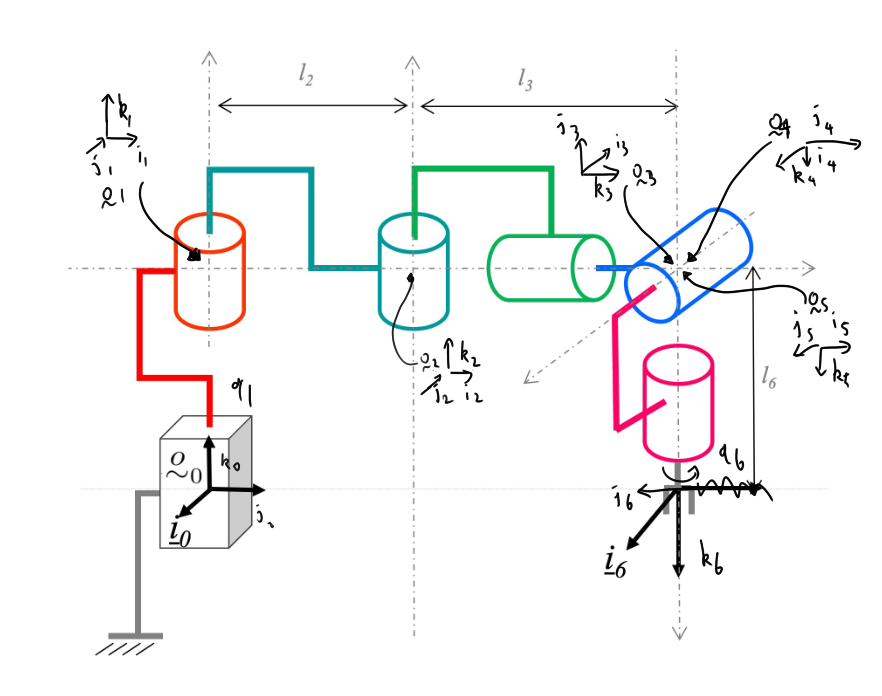
\includegraphics[width=120mm]{imgs/y2023-v1-q2.png}
    \end{center}

    \begin{center}
        \begin{tabular}{lllll}
               & $\theta$           & $d$   & $a$   & $\alpha$ \\
            j0 & $\pi/2$            & $d_1$ & 0     & 0        \\
            j1 & $\theta_2$         & 0     & $l_2$ & 0        \\
            j2 & $\pi/2+\theta_3$   & 0     & $l_3$ & $\pi/2$  \\
            j3 & $ -\pi/2+\theta_4$ & 0     & 0     & $\pi/2$  \\
            j4 & $\pi/2+\theta_5$   & 0     & 0     & $\pi/2$  \\
            j5 & $\pi/2$            & $l_6$ & 0     & 0        \\
        \end{tabular}
    \end{center}

    \begin{align*}
        {\,^0T_1} & =
        \begin{bmatrix}
            [e^{\frac{\pi}{2} k \times}] & [d_1 k] \\
            [0]                          & 1
        \end{bmatrix}
    \end{align*}

    \begin{align*}
        {\,^1T_2} & =
        \begin{bmatrix}
            [e^{\theta_2 k \times}] & [0] \\
            [0]                     & 1
        \end{bmatrix}
        \begin{bmatrix}
            [I_3] & [l_2 i] \\
            [0]   & 1
        \end{bmatrix} \\
                  & =
        \begin{bmatrix}
            [e^{\theta_2 k \times}] & [e^{\theta_2 k \times} \cdot l_2 i    ] \\
            [0]                     & 1
        \end{bmatrix}
    \end{align*}

    \begin{align*}
        {\,^2T_3} & =
        \begin{bmatrix}
            [e^{(\pi/2+\theta_3) k \times}] & [0] \\
            [0]                             & 1
        \end{bmatrix}
        \begin{bmatrix}
            [e^{(\pi/2) i \times}] & [l_3 i] \\
            [0]                    & 1
        \end{bmatrix} \\
                  & =
        \begin{bmatrix}
            [e^{(\pi/2+\theta_3) k \times}e^{(\pi/2) i \times}] & [e^{(\pi/2+\theta_3) k \times} l_3 i] \\
            [0]                                                 & 1
        \end{bmatrix}
    \end{align*}

    \begin{align*}
        {\,^3T_4} & =
        \begin{bmatrix}
            [e^{(-\pi/2. +\theta_4) k \times}] & [0] \\
            [0]                                & 1   \\
        \end{bmatrix}
        \begin{bmatrix}
            [e^{(\pi/2) i \times}] & [0] \\
            [0]                    & 1
        \end{bmatrix} \\
                  & =
        \begin{bmatrix}
            [e^{(-\pi/2. +\theta_4) k \times}e^{(\pi/2) i \times}] & [0] \\
            [0]                                                    & 1   \\
        \end{bmatrix}
    \end{align*}

    \begin{align*}
        {\,^4T_5} & =
        \begin{bmatrix}
            [e^{(\pi/2. +\theta_5) k \times}] & [0] \\
            [0]                               & 1   \\
        \end{bmatrix}
        \begin{bmatrix}
            [e^{(\pi/2) i \times}] & [0] \\
            [0]                    & 1
        \end{bmatrix} \\
                  & =
        \begin{bmatrix}
            [e^{(\pi/2. +\theta_5) k \times}e^{(\pi/2) i \times}] & [0] \\
            [0]                                                   & 1   \\
        \end{bmatrix}
    \end{align*}

    \begin{align*}
        {\,^5T_6} & =
        \begin{bmatrix}
            [e^{\pi/2 k \times}] & [l_6 k] \\
            [0]                  & 1
        \end{bmatrix}
    \end{align*}
\end{solutionbox}

\begin{solutionbox}[Q2-2]
    \footnotesize
    \begin{align*}
        J & =
        \begin{bmatrix}
            k_0                              &
            k_1 \times (\ppori{6}-\ppori{1}) &
            k_2 \times (\ppori{6}-\ppori{2}) &
            k_3 \times (\ppori{6}-\ppori{3}) &
            k_4 \times (\ppori{6}-\ppori{4}) &
            k_5 \times (\ppori{6}-\ppori{5})   \\
            0                                &
            k_1                              &
            k_2                              &
            k_3                              &
            k_4                              &
            k_5
        \end{bmatrix}
    \end{align*}


    since this is a spherical wrist, the wrist and the arm can be analyzed separately.

    \begin{align*}
        \begin{bmatrix}
            [I_3] & (\ppori{6}-\ppori{3})\times \\
            [0]   & [I_3]
        \end{bmatrix}
        J & =
        \begin{bmatrix}
            k_0                              &
            k_1 \times (\ppori{3}-\ppori{1}) &
            k_2 \times (\ppori{3}-\ppori{2}) &
            0                                &
            0                                &
            0                                  \\
            0                                &
            k_1                              &
            k_2                              &
            k_3                              &
            k_4                              &
            k_5
        \end{bmatrix}
    \end{align*}


    When $\theta_3 = 0$ or $\theta_3 = \pi$, joint 2 and joint 3 have the same effect, so it is a singularity.
    (I forgot this in previous practices.)

    When $\theta_5 = 0$ or $\theta_5=\pi$, joint 4 k axis and joint 6 k axis are aligned, so there effect are the same and is a singularity.

    (the following are probably not right since i'm not sure what suitable means here)

    yes, if the tasks arein one plane, then the first joint does't need to move and saves power. and if all of tasks are in a cylinedarical surface, it would line up with the first two degrees of freedom of the robot.


    The reachable workspace is a cylinder with height equal tot he rang eof the prismatic joint and radius l2, l3, l6, plus two capsules on top and bottom with height l6 flat region bounded outside by l3, bounded inside by radius equal to difference of l2 and l3.

    the dexerous workspace is a cylinder with height therange of the prismatic joint, and radius equal to l2+l3 - l6. th einside is more complicated. for a unreachable radius of |l2-l3|. |l2-l3|+l6 is not dexerous. top and bottom is too messy.

\end{solutionbox}

\begin{solutionbox}[Q2-3]

    walk back wads from o6 by k6 to get to wrist center.

    the height of the wrist center is where d1 is.

    the distance of the wrist center, as well as l2 and l3, can be passed into kahan 4 to solve for theta 3.

    mean of theta 2 can be found with kahan 2 rotating from i2 to o3-o1 using k0.

    using pi minus kahan 4 using a being the magneitude of o3-o1 as a, l2 as b, and l3 as c solves for theta 2 delta.

    both theta 2 delta and theta 3 are plus minus version but theta2 delta and theta 3 should have opposite sign. so the solution space branched into 2.

    project k6 onto i3 and j3 and normalize. the use kahan 2 from j3 to projected k6 around k3 gives one solution for theta 4, adding pi gives another solution for theta 4. so now the solution space has branched into 4.

    given variable up to theta 4, using kahan 2 from i5 to k5 using k4 gives the angle for theta 5. this is unique up to mod 2pi.

    then rotating from j5 to i6 across k5 gives theta 6. also unique.


\end{solutionbox}

\begin{solutionbox}[Q2-4]
    See 2025-v1-q2 last question
\end{solutionbox}

\newpage
\section{Exam 2022}
bye.
I'll put this on github and we can crowd source a solution.
\newpage
\begin{solutionbox}[Q2-1]

\end{solutionbox}

\begin{solutionbox}[Q2-2]
    \begin{align*}
        {\,^0C_1} & =e^{\theta_1 k \times} e^{ \frac{\pi}{2} i \times} \\
        {\,^1C_2} & =e^{\theta_2 k \times} e^{-\frac{\pi}{2} i \times} \\
        {\,^2C_3} & =e^{-\frac{\pi}{2} k \times}
    \end{align*}

    \begin{align*}
        \pv{\omega}_{3,0}  & = \dot{\theta}_1 \pv{k}_0 + \dot{\theta}_2 \pv{k}_1                                                      \\
        {\,^1\omega_{3,0}} & = \dot{\theta}_1 {\,^0C_1}^{T} k + \dot{\theta}_2 k                                                      \\
        {\,^1\omega_{3,0}} & = \dot{\theta}_1 \left[e^{\theta_1 k \times} e^{ \frac{\pi}{2} i \times}\right]^{T} k + \dot{\theta}_2 k \\
        {\,^1\omega_{3,0}} & = \dot{\theta}_1 \left[e^{ -\frac{\pi}{2} i \times} e^{-\theta_1 k \times}\right] k + \dot{\theta}_2 k   \\
        {\,^1\omega_{3,0}} & = \dot{\theta}_1 e^{ -\frac{\pi}{2} i \times} e^{-\theta_1 k \times} k + \dot{\theta}_2 k                \\
    \end{align*}
\end{solutionbox}


\newpage
\begin{solutionbox}[Q3-1]

    \begin{center}
        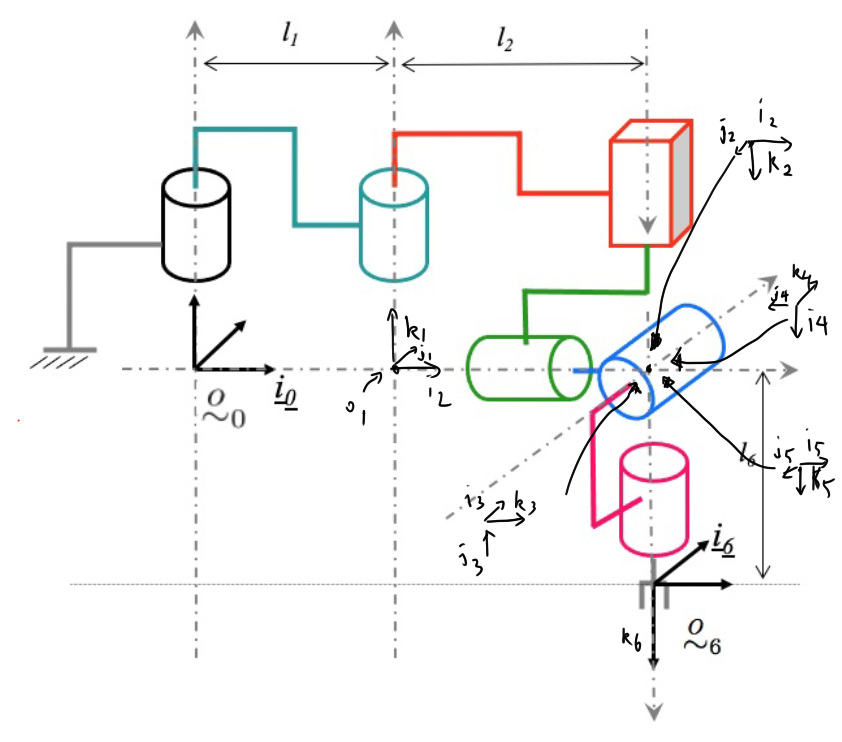
\includegraphics{imgs/y2022-v1-q3-1.png}
    \end{center}

    I don't think I actually need to generate DH table for this?

    Coordinate free form, very standard axis.

    Singularity when $\theta_2=0$ or $\pi$ which is elbow singularity. And when $\theta_5 =\pi/2$ or $3\pi/2$ which is a wrist singularity
\end{solutionbox}

\begin{solutionbox}[Q3-2]
    Walk back from o6 by k3 l6 to find o3.

    Project o3-o0 to plane perpendicular to k3.

    Use Kahan p4 to find theta 2 and theta 1. There is a branching here.

    Project o3-o0 onto k3, this is d3.

    With first three, C3 is known.

    $\pv{k}_4 = \pm \pv{k}_3\times \pv{k}_6 k4$ There is branching here.

    Use Kahan p2 to rotate i3 to k4 through k3 gives theta 4.

    Use Kahan p2 to rotate i4 to k5 through k4 gives theta 5.

    Use Kahan p2 to rotate i5 to j6 though k5 gives theta 6.

\end{solutionbox}
\newpage
\input{sections/y2022-v1-q4.tex}

\end{document}							%End of the document. 
